\documentclass{ximera}


%\addPrintStyle{../..}

\begin{document}
	\author{Bart Lambregs}
	\xmtitle{Het referentiestelsel}{}
    \xmsource\xmuitleg
 
Als je een vogel ziet vliegen, kan je deze beweging op verschillende manieren beschrijven: de vogel kan \textit{stijgen} of een \textit{duikvlucht} nemen. De vogel kan \textit{omdraaien} of -- indien het een kolibrie is -- misschien zelfs op een vaste plaats \textit{blijven fladderen}. Al deze beschrijvingen gebeuren met een referentiepunt in het achterhoofd. Je kan alleen maar stijgen ten opzichte van iets anders.

Elk bewegend systeem wordt sluitend beschreven ten opzichte van een \textbf{referentiestelsel}. Dat is een assenstelsel dat als het ware in de ruimte geplaatst wordt en waarin bijvoorbeeld de positie kan worden vastgelegd. Ten opzichte van dit stelsel kan je de plaats met een positievector beschrijven en een snelheidsvector gebruiken om de snelheid te beschrijven.
% Definitie van referentiestelsel zou nog een kader moeten krijgen ...

De keuze van het referentiestelsel is altijd \textit{vrij}. Het is belangrijk om die keuze telkens duidelijk te maken. Stel je voor dat je op dit moment gedreven natuurkunde aan het studeren bent aan een bureau en je houdt je pen op \textit{ooghoogte}, hoe `hoog' bevindt je pen zich dan? Meet je dit vanaf je tafelblad, de vloer, het straatniveau, het aantal meters boven de zeespiegel, ...? In welke eenheid meet je dit? Wat is je eenheidsvector en in welke richting kies je de positieve as? 

Meestal wordt geopteerd voor een referentiestelsel dat stilstaat. %waarvoor de 'waarnemer' stilstaat. % footnote bewegende referentiestelsels --> speciale relativiteit  % Waarnemer moet ook uitgelegd worden ...
In onderstaand voorbeeld van het voetbalveld is de positie \(\vec{r}\) van de voetballer duidelijk verschillend naargelang het gekozen referentiestelsel.

%Voor een toeschouwer in het publiek staan beide referentiestelsels stil, bijgevolg is de snelheid \(\vec{v}\) voor beiden dezelfde. = toeschouwer is opnieuw een andere keuze van een referentiestelsel. Zonder dat te benoemen vind ik het verwarrend. = als snelheid een gebonden vector is, is die vector voor de verschillende keuzes verschillend ...?


\begin{center}
\begin{minipage}[t]{0.70\textwidth}
\begin{image}[\linewidth]
	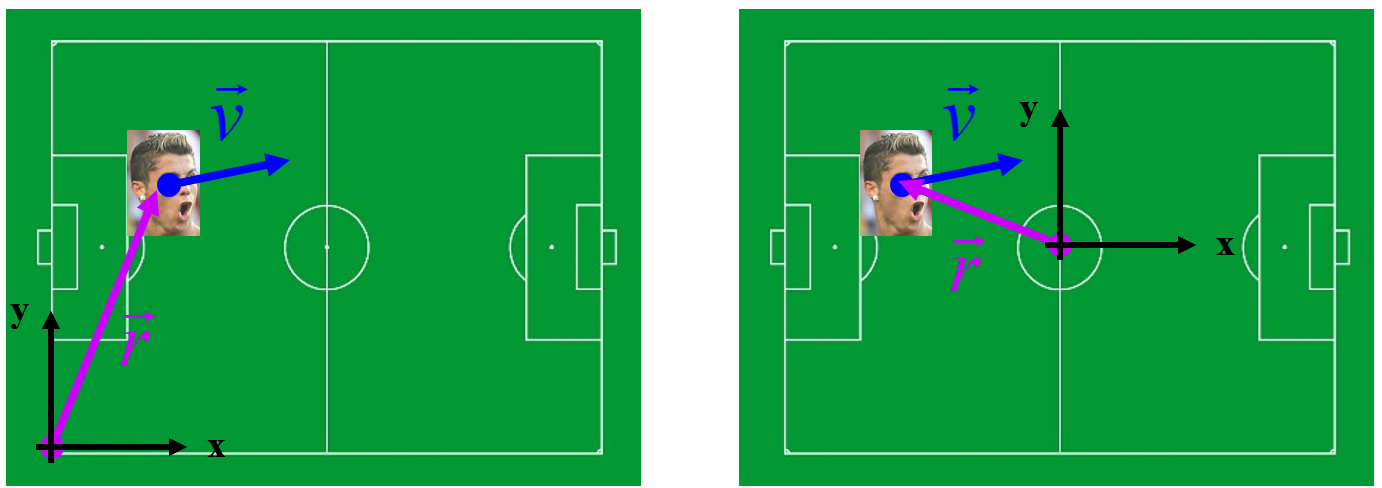
\includegraphics{referentiestelsels}
% Uit ppt Vincent, IK WIL AFBEELDING GROTER MAAR LUKT ME NIET.
\end{image}
\end{minipage}
\end{center}
\captionof{figure}{Twee verschillende referentiestelsels}


\begin{exercise}
De kolibrie in onderstaande foto blijft ter plekke in de lucht fladderen onder de bloem. Geef twee referentiestelsels waarin deze vogel \textbf{niet} stilstaat. 

\begin{center}
\begin{minipage}[t]{0.30\textwidth}
\begin{image}[\linewidth]
	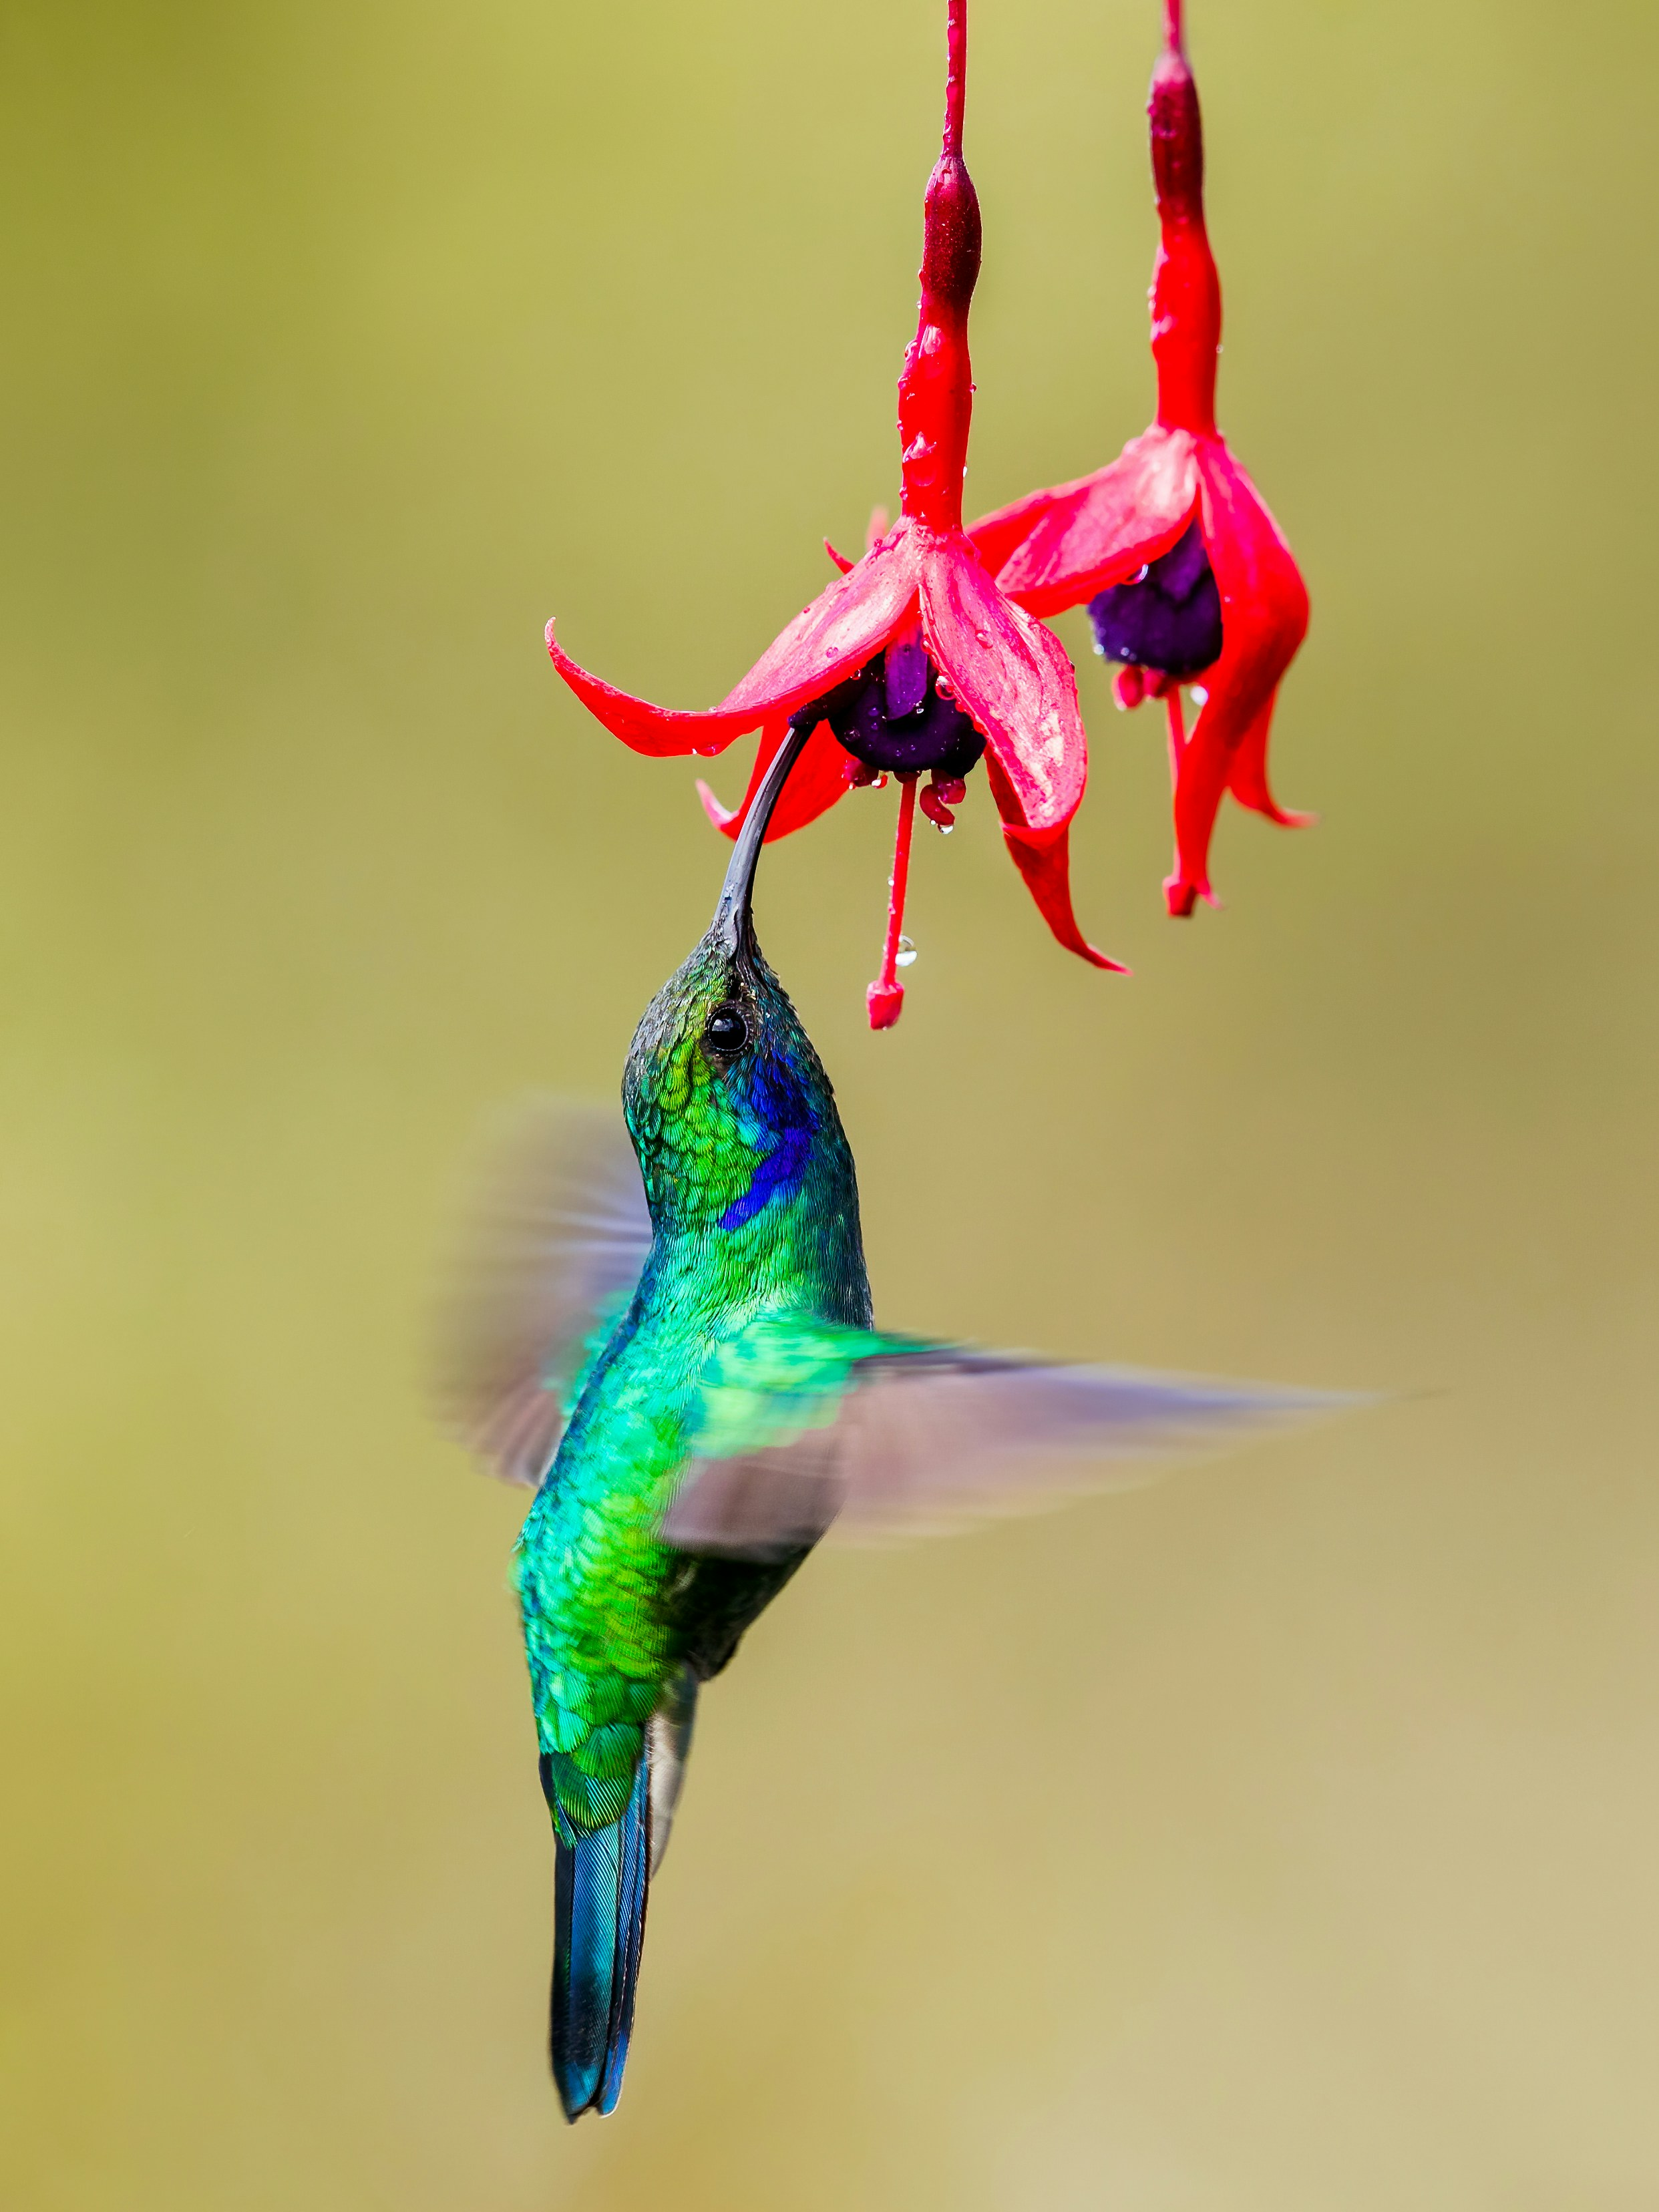
\includegraphics{kolibri}
% Bron: https://unsplash.com/photos/green-and-black-humming-bird-flying-p-DDK9lOmmE 
\end{image}
\end{minipage}
\end{center}


\begin{oplossing}\nl
\begin{itemize}
\item Een referentiestelsel met de kern van de aarde als oorsprong. (De kolibrie draait nu rond de as van de aarde...)
\item Een referentiestelsel met de zon als middelpunt (De kolibrie draait nu ook rond de zon...)
\end{itemize}

\end{oplossing}

\end{exercise}


\end{document}

% Volgende elementen veranderde ik in de tekst, last minute. Met kans op iets fout te doen natuurlijk ...

%Deze omvat een assenstelsel met een oorsprong (= het \textbf{referentiepunt}).
%Binnen dit referentiestelsel worden de vectoriële grootheden beschreven waaruit de kinematica is opgebouwd. 
%Om deze bewegingen kwantitatief te beschrijven, kies je dus een referentiestelsel. 
%Op die manier krijgt de vogel een positievector die de positie aangeeft, een snelheidsvector die de snelheid aangeeft, ... 
% en coördinaatassen. %Bart: coördinaatassen hier vermelden overbodig of niet? 
% ...




